\documentclass{article}
\usepackage[utf8]{inputenc}
\usepackage{amsmath}
\usepackage{amssymb}
\usepackage{amsthm}
\usepackage{cancel}
\usepackage[shortlabels]{enumitem}
\usepackage{caption}
\usepackage{graphicx}
\usepackage[top=0.5in, bottom=0.5in, left=1in, right=1in]{geometry}
\usepackage{float}

% \usepackage{titlesec}
%     \titlespacing{\subsection}{\parindent}{15pt}{12pt}

\title{\textbf{\underline{CSCI4150U: Data Mining}\\Lab 03}}
\author{Syed Naqvi\\100590852}
\date{\today}

\begin{document}

    \maketitle
    
    \section*{Part I:}

    \subsection*{1.}

    Average and individual trial results across 5 randomized trials using accuracy, precision and f1 scores as performance metrics based on
    a (90\%-train and 10\%-test) \textbf{holdout} validation method, decision tree classifiers and Gini impurity.

    \begin{figure}[H]
        \centering
        \begin{minipage}[t]{0.47\textwidth}
            \centering
            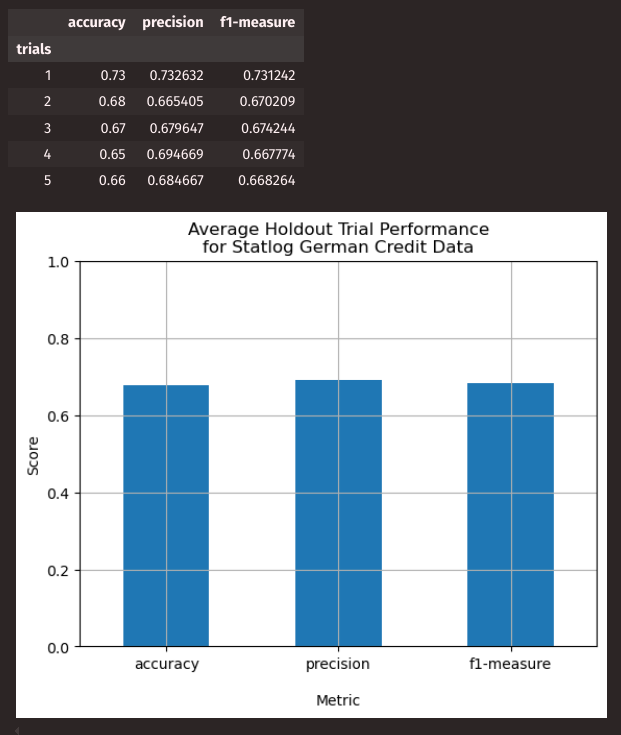
\includegraphics[width=\textwidth, height=0.35\textheight]{1hg.png}
            \caption{Decision tree performance based on holdout method and Gini impurity using Statlog German Credit Dataset}
        \end{minipage}
        \hfill
        \begin{minipage}[t]{0.47\textwidth}
            \centering
            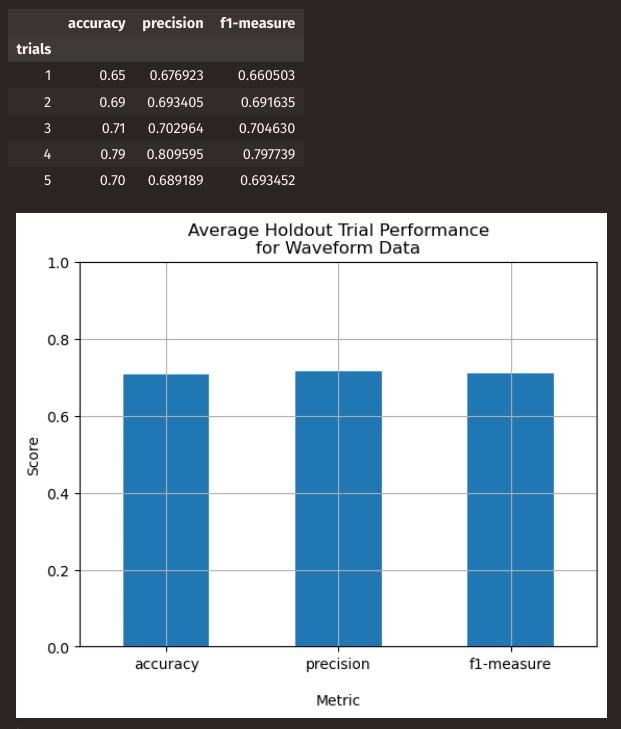
\includegraphics[width=\textwidth, height=0.35\textheight]{1hw.png}
            \caption{Decision tree performance basd on holdout method and Gini impurity using Waveform Dataset}
        \end{minipage}
    \end{figure}

    \newpage

    \subsection*{2.}

    Average and individual trial results using accuracy, precision and f1 scores based on \textbf{10-fold cross-validation}, decision tree
    classifiers and Gini impurity.

    \begin{figure}[H]
        \centering
        \begin{minipage}[t]{0.47\textwidth}
            \centering
            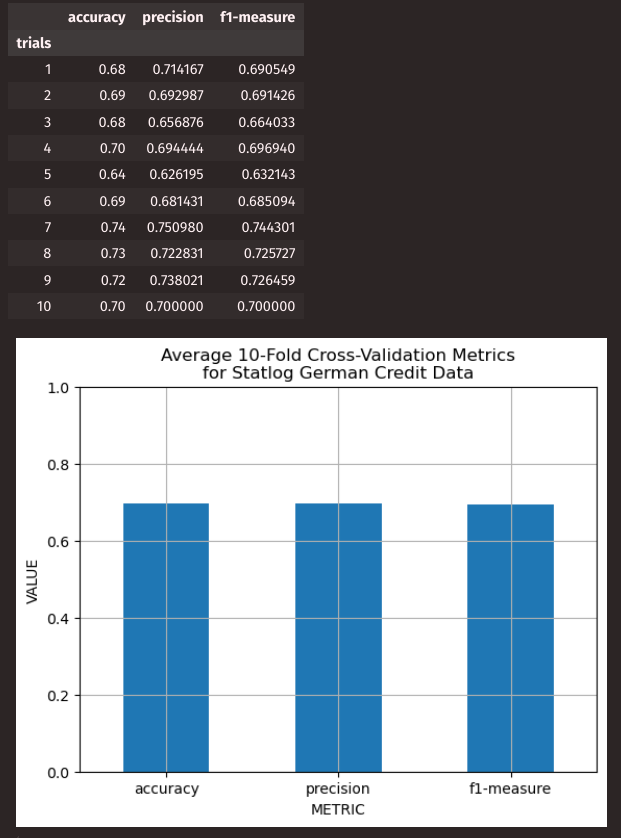
\includegraphics[width=\textwidth, height=0.35\textheight]{1cg.png}
            \caption{Decision tree performance based on 10-fold cross-validation and Gini impurity using Statlog German Credit Dataset}
        \end{minipage}
        \hfill
        \begin{minipage}[t]{0.47\textwidth}
            \centering
            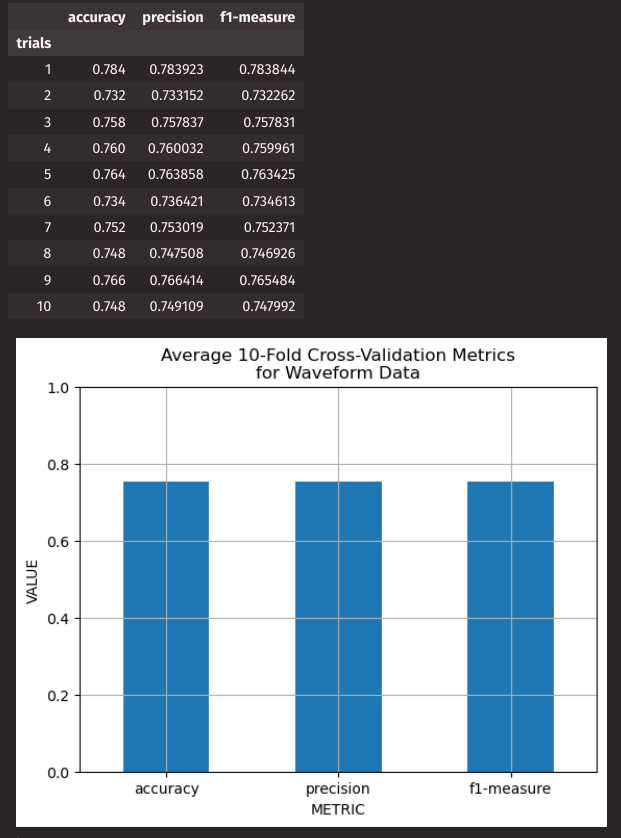
\includegraphics[width=\textwidth, height=0.35\textheight]{1cw.png}
            \caption{Decision tree performance based on 10-fold cross-validation and Gini impurity using Waveform Dataset}
        \end{minipage}
    \end{figure}

    \newpage

    \section*{Part II:}

    \subsection*{1.}

    Repetition of \textbf{Part I}, this time using \textbf{'Entropy'} instead of \textbf{'Gini;} as the decision-tree impurity measure.

    \begin{figure}[H]
        \centering
        \begin{minipage}[t]{0.47\textwidth}
            \centering
            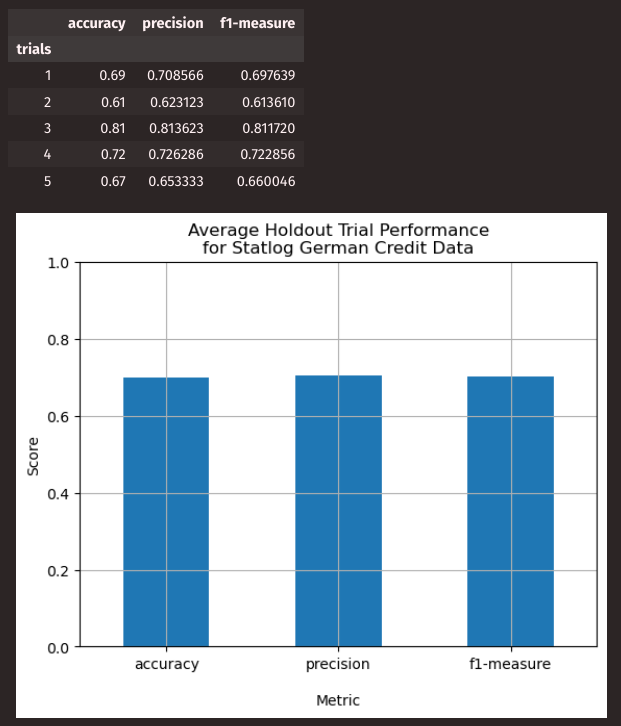
\includegraphics[width=\textwidth, height=0.35\textheight]{2hg.png}
            \caption{Decision tree performance based on holdout method and Entropy impurity using Statlog German Credit Dataset}
        \end{minipage}
        \hfill
        \begin{minipage}[t]{0.47\textwidth}
            \centering
            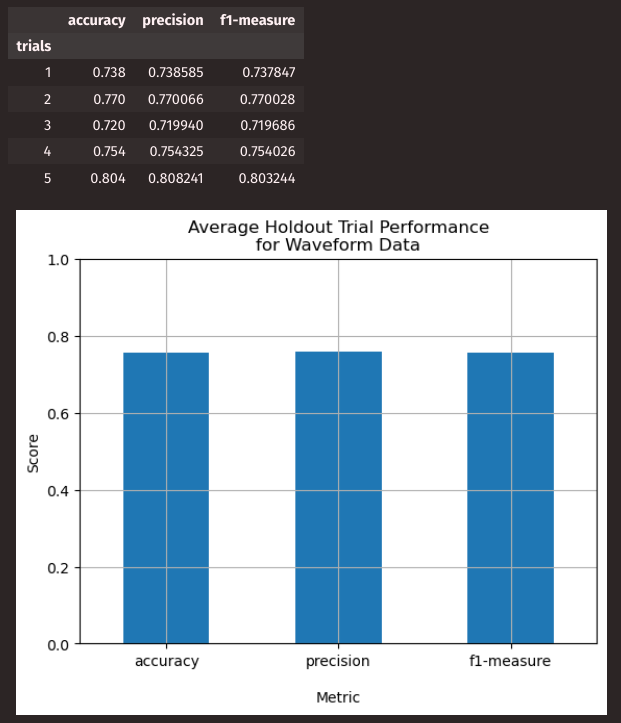
\includegraphics[width=\textwidth, height=0.35\textheight]{2hw.png}
            \caption{Decision tree performance based on holdout method and Entropy impurity using Waveform Dataset}
        \end{minipage}
        
    \end{figure}

    \begin{figure}[H]
        \centering
        \begin{minipage}[t]{0.47\textwidth}
            \centering
            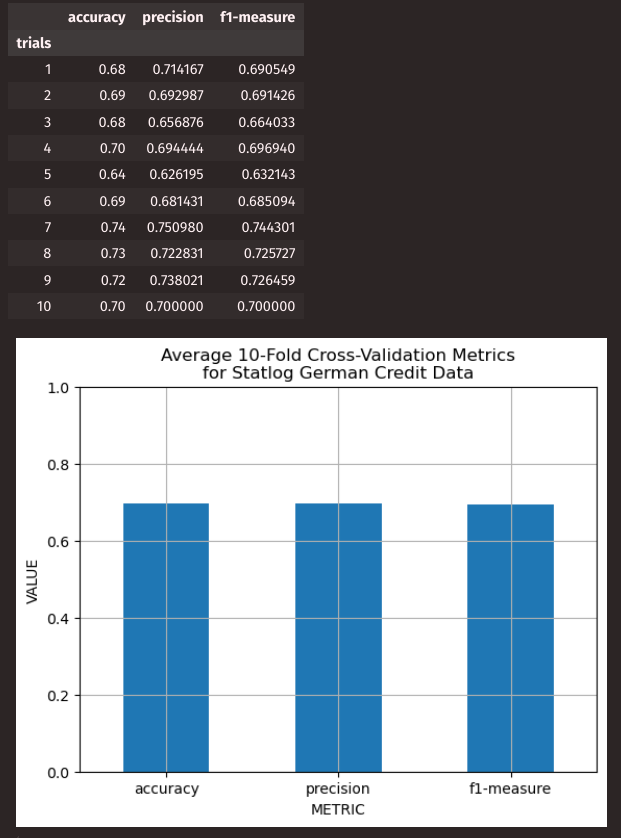
\includegraphics[width=\textwidth, height=0.35\textheight]{1cg.png}
            \caption{Decision tree performance based on 10-fold cross-validation and Entropy impurity using Statlog German Credit Dataset}
        \end{minipage}
        \hfill
        \begin{minipage}[t]{0.47\textwidth}
            \centering
            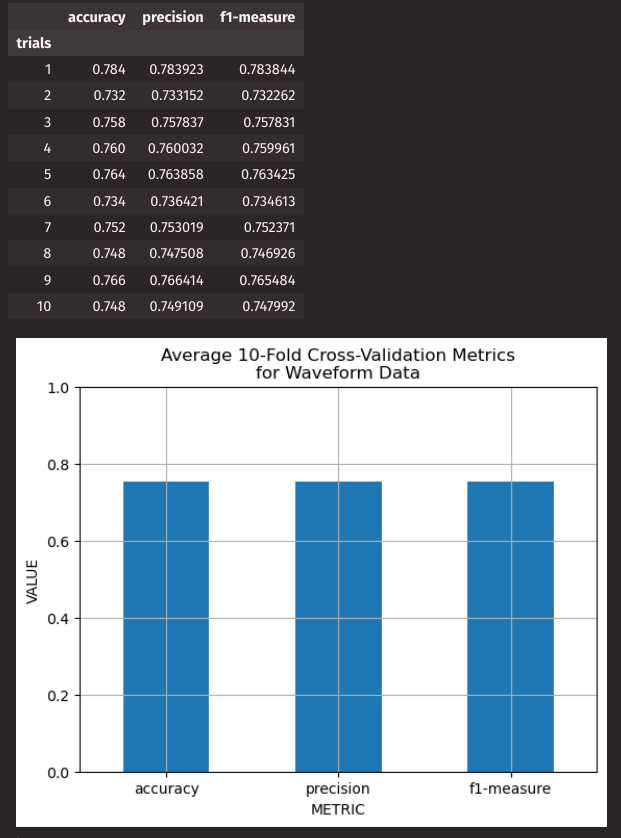
\includegraphics[width=\textwidth, height=0.35\textheight]{1cw.png}
            \caption{Decision tree performance based on 10-fold cross-validation and Entropy impurity using Waveform Dataset}
        \end{minipage}
    \end{figure}

    \newpage

    \subsection*{2.}

    Comparing the average \textbf{10-fold cross-validation} based accuracy of decision-tree classifiers using \textbf{'Gini'}
    vs \textbf{'Entropy'} as impurity measures for both \textbf{Statlog German Credit} and \textbf{Waveform Datasets}.

    \begin{figure}[H]
        \centering
        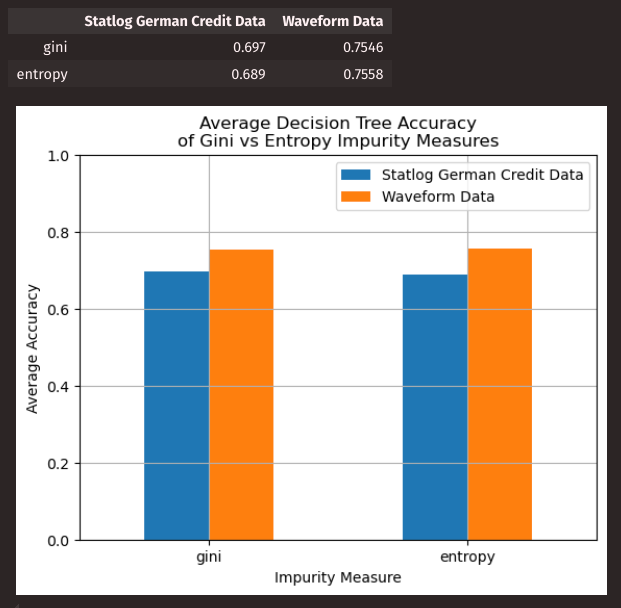
\includegraphics[width=\textwidth, height=0.6\textheight]{2comparison.png}
        \caption{Accuracy comparison of decision tree classifiers using Entropy vs Gini impurity measures}
    \end{figure}

    \newpage

    \section*{Part III:}

    \subsection*{1.}

    Plotting decision tree accuracies based on the (90\%-train and 10\%-test) \textbf{holdout} validation method and varying max tree depths.

    \begin{figure}[H]
        \centering
        \begin{minipage}[t]{0.47\textwidth}
            \centering
            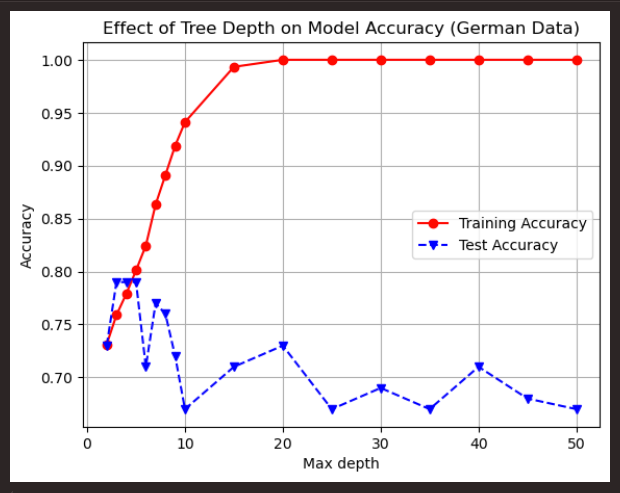
\includegraphics[width=\textwidth, height=0.30\textheight]{3a.png}
            \caption{Decision tree accuracies for Statlog German Credit Dataset}
        \end{minipage}
        \hfill
        \begin{minipage}[t]{0.47\textwidth}
            \centering
            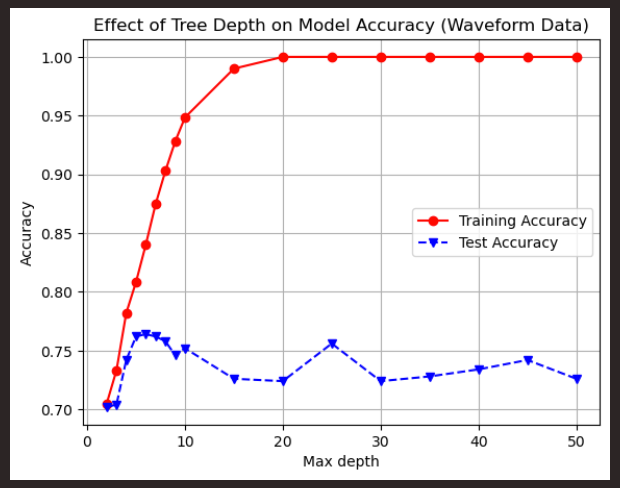
\includegraphics[width=\textwidth, height=0.30\textheight]{3b.png}
            \caption{Decision tree accuracies for Waveform Dataset}
        \end{minipage}
    \end{figure}

    \subsection*{2.}

    We can see clearly that with increasing tree depth there is an overfitting phenomenon observable across both datasets. The model achieves an
    increasingly better fit to its training data until it can perfectly classify all records. However, we see consistently that after a short
    period of increasing test accuracy, the model experiences a net decrease in test accuracy with increasing tree depth. This indicates that
    after a certain tree depth, the model starts to become highly specialized and overfits to its training data. This results in a model that poorly
    generalizes to unseen test data.

\end{document}